\section{Electronic Noise}
\begin{itemize}
    \itemsep0pt
    \item Noise: \textit{threshold for the perception of a signal}
    \item \textbf{Signal-to-noise ration:} \(\dfrac{S}{N} = \dfrac{P_S}{P_N}\)
    \item Limits of perceptibility:
        \begin{itemize}
            \item Analogue speech signal: $\text{NL} \approx 0\si{dB}$
            \item Analogue TV signal $\text{NL} \approx 34\si{dB}$
            \item With apriori and correlation techniques \(\implies \text{NL} < 0\si{dB}\)
        \end{itemize}
    \item \textbf{Noise sources}:
        \begin{itemize}
            \item Thermal noise $\propto T$ (resistors)
            \item Shot noise $\propto q_e I_{DC}$ (active/biased elements)
            \item Antenna noise: man-made, atmospheric (lightning) and cosmic (CMB)
        \end{itemize}
\end{itemize}

\subsection{Properties of Noise Signals}
\begin{itemize}
    \item Temporal behaviour is fundamentally \textit{unpredictable} $\implies$ integral values are predictable:
        \begin{align*}
            &\text{Linear, time average:}\\
            &\bar{u}^{\Delta t} = \dfrac{1}{\Delta t}\int\limits^{t_0+\Delta t}_{t_0} u(t) \mathrm{d}t\\
            &\text{Mean square:}\\
            &\overline{u^2}^{\Delta t} = \dfrac{1}{\Delta t}\int\limits^{t_0+\Delta t}_{t_0} u^2(t) \mathrm{d}t\\
            &\text{Root Mean Square (RMS):}\\
            &\tilde{u}=\sqrt{\overline{u^2}}
        \end{align*}
    \item Wide sense stationarity assumed; $\bar{u}^{\Delta t}$ and $\overline{u^2}^{\Delta t}$ independant from $t_0$
    \item Spectral density of voltage: \(W_u^s = \left.\dfrac{\bar{u}^2}{\Delta f}\right|_{\Delta f \to 0}\)
    \item \textbf{Central Limit Theorem} (Gaussian PDF):
        \(p^*(u) = \dfrac{1}{\sqrt{2\pi\:\overline{u^2}}}\exp\left(- \dfrac{1}{2}\dfrac{u^2}{\overline{u^2}}\right)\)
    \item \textbf{(Normalized) Error Function:}
        \begin{align*}
            p(0<u<u_1) &= \int\limits_0^{u_1} p^*(u)\mathrm{d}u =\\
            &= \Phi^*\left(\dfrac{u_1}{\tilde{u}}\right) \approx \dfrac{1}{2} - \dfrac{\exp(-\frac{1}{2}\frac{u_1^2}{\tilde{u}^2})}{\sqrt{2\pi}(u_1/\tilde{u})}
        \end{align*}
        \begin{tabular}{|c|c|c|c|c|}\hline
            $\dfrac{u_1}{\sqrt{\overline{u^2}}}$ & 1 & 2 & 3 & 4\\\hline
            $\Phi^*$ & 0.413 & 0.4772 & 0.4987 & 0.49997\\\hline
        \end{tabular}
\end{itemize}

\subsection{Working with Noise Signals}
\subsubsection{Correlation Functions}
\begin{itemize}
    \itemsep0pt
    \item Auto- ($i=j$)/Cross- ($i\neq j$)\textbf{Correlation Function}:
    \begin{align*}
        \rho_{ij}(\tau) &= \overline{u_i(t) u_j(t+\tau)}\\
        &= \lim_{\Delta t\to\infty} \dfrac{1}{\Delta t} \int\limits^{t_0+\Delta t}_{t_0} u_i(t) u_j(t+\tau) \mathrm{d}t
    \end{align*}
    \item $\rho_{ii}(\tau) = \rho_{ii}(-\tau) \implies \text{Even function!}$
    \item $\rho(0) = \sqrt{\overline{u^2}} = \tilde{u}$ (RMS)
    \item However, cross-correlation function $\rho_{ij}(\tau)$ \textit{not generally even!}
\end{itemize}

\subsubsection{Noise Signals in Frequency Domain}
\begin{align*}
    &\overline{u^2} = \int\limits_0^\infty W_u^s(f) \mathrm{d}f = |\tilde{u}|^2\\
    &W_u^s\text{: single-sided (power) spectral density}
\end{align*}
\begin{itemize}
    \itemsep0pt
    \item Double-sided spectral densities (\textit{even function}) as Fourier transform of correlation functions:
        \begin{align*}
            W_u(f) &= \int\limits^\infty_{-\infty}\rho(\tau)\,e^{-j2\pi f\tau}\mathrm{d}\tau\\
            &= \int\limits^\infty_{-\infty}\rho(\tau) \cos(-j2\pi f\tau)\mathrm{d}\tau\\
        \end{align*}
    \item \textbf{Wiener-Khinchin-Relations:}
    \begin{align*}
        &W_{u12} = \int\limits^\infty_{-\infty}\rho_{12}(\tau)\,e^{-j2\pi f\tau}\mathrm{d}\tau,\\
        &W_{u12}(f) = W_{u21}^*(f),\\
        &W_{u21}(f) = W_{u21}^*(-f)
    \end{align*}
    \item Normalized cross spectral density $\gamma$:
        \begin{equation*}
            \gamma = \dfrac{W_{u12}(f)}{\sqrt{W_u1(f)} \sqrt{W_u2(f)}}
        \end{equation*}
\end{itemize}

\subsubsection{Noise Signals in Linear Networks}
\begin{tabular}{cc}
    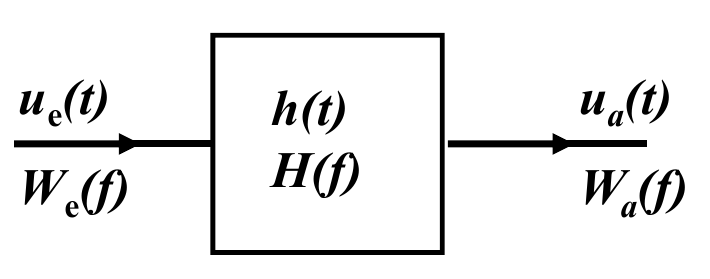
\includegraphics[width=3.5cm]{content/hfcomp/pictures/2-port_linear_network.png}\
    &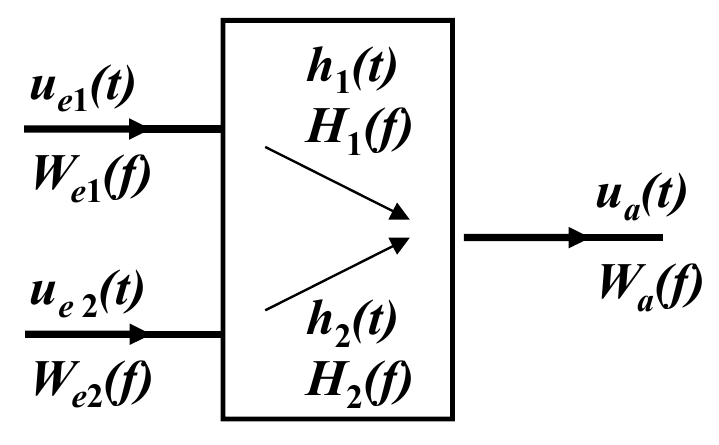
\includegraphics[width=3.5cm]{content/hfcomp/pictures/3-port_linear_network.png}\\
\end{tabular}
\begin{itemize}
    \itemsep0pt
    \item Two-port network with tranfer function $h(t)$:
        \begin{align*}
            &\rho_a(\tau) = \int\limits_{-\infty}^\infty\int\limits_{-\infty}^\infty\
            h(t')h(t'')\rho_e(\tau+t'-t'')\mathrm{d}t'\mathrm{d}t'',\\
            &W_a(f) = |H(f)|^2 W_e(f),\\
            &\rho_e\text{: Input autocorrelation function}\\
            &\rho_a\text{: Output autocorrelation function}
        \end{align*}
%    \item Three-port network (2 in-, 1 output) with tranfer functions $h_{1/2}(t)$:
%        \begin{align*}
%            W_a(f) = &|H_1(f)|^2 W_{e1}(f) + |H_2(f)|^2 W_{e2}(f)\\
%            &+ 2\:\mathrm{Re}\{H_1^*(f) H_2^*(f) W_{e1e2}(f)\}
%        \end{align*}
\end{itemize}
\fbox{%
    \parbox{7.5cm}{%
        \textbf{Symbolic Calculation of Noise Sources:}
        \begin{enumerate}
            \item Treat noise sources like normal current/voltage sources and apply Kirchhoff's laws to combine sources, e.g.
                \begin{equation*}
                    U_a = H_1(f)U_{e1} + H_2(f)U_{e2}.
                \end{equation*}
            \item Take the magnitude squared of the expression and apply the correspondence $|\tilde{U}_{e1}|^2 = W_{e1}$ for voltage or $|\tilde{I}_{e1}|^2 = W_{e1}$ for current sources, e.g.
                \begin{align*}
                    |U_a|^2 = &|H_1|^2|U_{e1}|^2 + |H_2|^2|U_{e2}|^2\\
                    &+ 2\:\mathrm{Re}\{H_1^* H_2^*\:U_{e1}^* U_{e2}\},\\
                    \updownarrow\\
                    W_a(f) = &|H_1|^2 W_{e1} + |H_2|^2 W_{e2}\\
                    &+ 2\:\mathrm{Re}\{H_1^* H_2^*\:W_{e1e2}\}.
                \end{align*}
        \end{enumerate}}
    }

\subsection{Noise of Two-Terminal Elements}
\subsubsection{Thermal Noise}
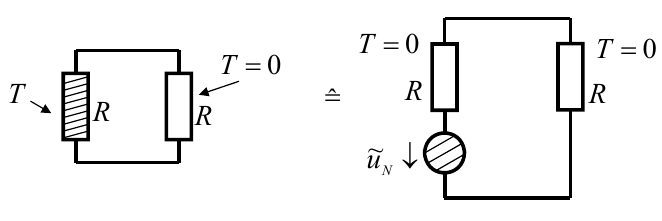
\includegraphics[width=.33\paperheight]{content/hfcomp/pictures/thermal_noise_resistor.png}
\begin{align*}
    &\overline{u^2(t)} = 4k_B T R\,\Delta f = |\tilde{u}|^2\\
    &W_{tu}^s(f) = 4\,k_B T\,R \quad \text{(single-sided)}\\\\
    &P_{N\;\mathrm{max}} = \dfrac{\overline{u^2(t)}}{4}\dfrac{1}{R} = k_B T\Delta f\\
    &\dfrac{P_{N\;\mathrm{max}}}{\mathrm{W}} = 4\cdot10^{-21}\;\dfrac{\Delta f}{\mathrm{Hz}}\dfrac{T}{T_0}
\end{align*}

\subsubsection{Noise of Receiving Antennas}
\begin{itemize}
    \itemsep0pt
    \item Equivalent antenna noise temperature $T_a=T$ (like a \textit{black body})
    \item Sources:
        \begin{itemize}
            \itemsep0pt
            \item cosmic noise
            \item atmospheric noise (tropical thunderstorms)
            \item ionospheric (fluctuation) noise
            \item heat radiation of the earth received by low directivity antennas
        \end{itemize}
\end{itemize}

\subsubsection{Shot Noise}
\begin{itemize}
    \itemsep0pt
    \item Due to the \textit{quantisation of electric charge}
    \item \textbf{Shottky equation} (derived from considering high vacuum diode):
        \begin{align*}
            W_{is}^s(f) = 2q_e\,q_e n |S(f)|^2 \approx 2 q_e\,I_{\mathrm{DC}}
        \end{align*}
\end{itemize}

\subsection{Noise of Diodes}
\begin{center}
    \begin{circuitikz}[scale=.8, transform shape]
    \begin{scope}[scale=1.2, xshift=-1cm]
        \draw (0,0) to[stroke diode, v=$u$, i=$i$, o-o] (2,0);
    \end{scope}
    \begin{scope}[xshift=2cm, yshift=-1cm]
        \draw (4,2)node[ocirc]{}
        -- (0,2)
        to[R=$G_S$] (0,0)
        -- (4,0)node[ocirc]{};
        \draw (2, 2) to[european current source, l=$W_{i,s}^s$, i<=$\tilde{I}$, fill=gray!50, *-*] (2,0);
    \end{scope}
\end{circuitikz}
\\
    \textit{Schottky diode and equivalent noise circuit.}
\end{center}
\begin{itemize}
    \item Diode noise power:
    \begin{equation*}
        W_{i,s}^s = 2\,q_e (I_0 + 2I_{ss}), \quad I_{ss}\text{: sat. current}
    \end{equation*}
\end{itemize}

\subsection{Noise of Two-Ports}
\begin{itemize}
    \item Transducer Power Gain:
        \begin{equation*}
            g_T = \dfrac{P_{\mathrm{out}}}{P_{\mathrm{in},\mathrm{max}}} = |A_B|^2
        \end{equation*}
    \item Two-port's noise as an effective thermal noise source ($T_z$)
    \item \textit{Noise Figure} $F$, as ratio of input- and output-SNR:
        \begin{align*}
            &F = \dfrac{T_0 + T_z}{T_0} = 1 + \dfrac{T_z}{T_0} = 1 + F_z\\
            &F_z\text{: excess noise figure}\\
            &T_0\text{: real temperature}
        \end{align*}
    \item \textbf{Noise of a passive two-port}:
        \begin{equation*}
            T_z = \dfrac{(1 - g_T)}{g_T}\,T_0
        \end{equation*}
    \item Cascade of $n$ two-ports:
        \begin{equation*}
            F_z = F_{z1} + \dfrac{F_{z2}}{g_{T1,\mathrm{max}}} +\dots+\dfrac{F_{zn}}{\prod\limits_{i=1}^{n-1}g_{Ti,\mathrm{max}}}
        \end{equation*}
    \item \textit{First amplifier} in a cascade of noisy two-port should have a \textit{low noise figure}!
    \item Noise Measure $M_i$:
        \begin{equation*}
            M_i = \dfrac{F_{zi}}{1 - \dfrac{1}{g_{Ti,\mathrm{max}}}}
        \end{equation*}
\end{itemize}
\subsubsection{Noise of Bipolar Transistor}
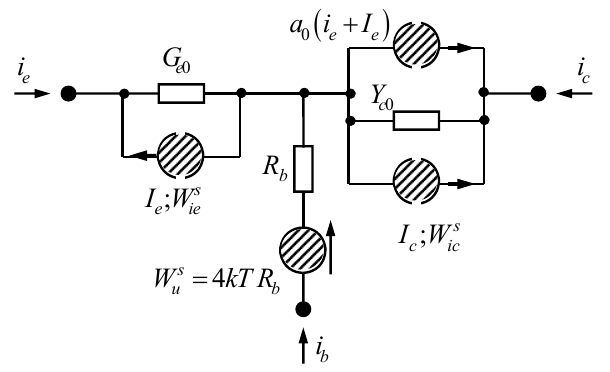
\includegraphics[width=.3\textwidth]{content/hfcomp/pictures/bjt_noise_circuit.png}
\begin{align*}
    &i_e = I_{ee} \left[\exp\left(\dfrac{q_e u_{eb}}{k_B T}\right) - 1\right] \quad \text{(signal current)},\\
    &W_{ie}^s =
    \begin{cases}
        4k_B T G_{e0} - 2q_e I_{ee} \approx 2k_B T G_{e0}, \quad I_{ee} \ll I_{eDC},\\
        2q_e (I_{eDC} + 2 I_{ee}) \equiv |\tilde{I}_e|^2, \quad \text{else}
    \end{cases}\\
    &W_{ic}^s = 2q_e a_0 (I_{eDC} + I_{ee}) + 2q_e I_{cc} \equiv |\tilde{I}^c|^2
\end{align*}
\subsubsection{Noise Matching}
\begin{itemize}
    \item \textbf{Goal:} Choose an internal generator impedance $Z_i=R_i + jX_i$ that minimizes the noise figure of a noisy two-port.
    \item Assume input noise sources:
        \begin{align*}
            &|\tilde{U}_{Nu}|^2 = 4k_B T_0 R_n \Delta f,\\
            &|\tilde{I}_{N}|^2 = 4k_B T_0 G_n \Delta f,\\
            &\tilde{U}_{Nc} = Z_c \tilde{I}_N, \quad Z_c=R_c + jX_c,\\
            &(\tilde{U}_{Nu}\text{ and }\tilde{I}_N\text{ uncorrelated})
        \end{align*}
    \item We get the optimal $Z_{i,\mathrm{opt}}$ minimal noise figure $F_{z,\mathrm{min}}$:
        \begin{align*}
            &R_{i, \mathrm{opt}} = \sqrt{\dfrac{R_n}{G_n} + R_c^2},\quad X_{i, \mathrm{opt}} = -X_c,\\
            &F_{z,\mathrm{min}} = 2\left[G_n R_n + \sqrt{G_n R_c + (G_n R_c)^2}\right]
        \end{align*}
    \item Circles of constant noise figure:
        \begin{align*}
            &\rho = \dfrac{Z_i - Z_{\mathrm{opt}}}{Z_i + Z_{\mathrm{opt}}^*}, \quad
            \Delta F = G_n R_{\mathrm{opt}},\\
            &F_z = F_{z,\mathrm{min}} \Delta F \dfrac{4|\rho|^2}{1 - |\rho|^2},\\
            &|\rho| = \sqrt{(F_z - F_{z,\mathrm{min}}) / (F_z + 4\Delta F - F_{z,\mathrm{min}})}\\
        \end{align*}
\end{itemize}
